\documentclass[11pt]{article}
% Shared preamble for the pyMack LST documentation set.
% Used by: mean_boundary_layer.tex, disturbance_equations.tex,
%          numerical_methods.tex, validation.tex
% Each document begins with:  \documentclass[11pt]{article}% Shared preamble for the pyMack LST documentation set.
% Used by: mean_boundary_layer.tex, disturbance_equations.tex,
%          numerical_methods.tex, validation.tex
% Each document begins with:  \documentclass[11pt]{article}% Shared preamble for the pyMack LST documentation set.
% Used by: mean_boundary_layer.tex, disturbance_equations.tex,
%          numerical_methods.tex, validation.tex
% Each document begins with:  \documentclass[11pt]{article}\input{lst_preamble}
\usepackage[margin=1in]{geometry}
\usepackage{amsmath,amssymb,mathtools}
\usepackage{booktabs}
\usepackage{enumitem}
\usepackage{array}
\usepackage{graphicx}
\usepackage{caption}
\usepackage{xcolor}
\usepackage[hidelinks]{hyperref}

\graphicspath{{figures/}}
\captionsetup{font=small,labelfont=bf}

\definecolor{kicol}{RGB}{31,143,107}
\definecolor{boxbg}{RGB}{238,246,242}
\definecolor{rmkbg}{RGB}{244,244,244}

\newcommand{\plain}[1]{\par\smallskip\noindent{\color{kicol}\textbf{In plain words.}}\ \textit{#1}\par\smallskip}
\newcommand{\problembox}[1]{%
  \par\smallskip\noindent\fcolorbox{kicol}{boxbg}{%
  \parbox{0.965\linewidth}{\smallskip\textbf{\color{kicol}What problem is solved here.}\ \ #1\smallskip}}\par\smallskip}
\newcommand{\remark}[2]{%
  \par\smallskip\noindent\colorbox{rmkbg}{%
  \parbox{0.965\linewidth}{\smallskip\footnotesize\textbf{#1}\ \ #2\smallskip}}\par\smallskip}
\newcommand{\bridge}[1]{\par\noindent\textit{#1}\par\medskip}

\newcommand{\D}{\mathrm{D}}
\newcommand{\imag}{\mathrm{i}}
\newcommand{\Real}{\operatorname{Re}}
\newcommand{\Imag}{\operatorname{Im}}
\newcommand{\Mae}{M_e}
\newcommand{\Ree}{\mathit{Re}}
\renewcommand{\bar}[1]{\overline{#1}}
\newcommand{\hatu}{\hat{u}}
\newcommand{\hatv}{\hat{v}}
\newcommand{\hatT}{\hat{T}}
\newcommand{\hatp}{\hat{p}}
\newcommand{\hatq}{\hat{q}}
\newcommand{\nuR}{\nu_{\!R}}

\usepackage[margin=1in]{geometry}
\usepackage{amsmath,amssymb,mathtools}
\usepackage{booktabs}
\usepackage{enumitem}
\usepackage{array}
\usepackage{graphicx}
\usepackage{caption}
\usepackage{xcolor}
\usepackage[hidelinks]{hyperref}

\graphicspath{{figures/}}
\captionsetup{font=small,labelfont=bf}

\definecolor{kicol}{RGB}{31,143,107}
\definecolor{boxbg}{RGB}{238,246,242}
\definecolor{rmkbg}{RGB}{244,244,244}

\newcommand{\plain}[1]{\par\smallskip\noindent{\color{kicol}\textbf{In plain words.}}\ \textit{#1}\par\smallskip}
\newcommand{\problembox}[1]{%
  \par\smallskip\noindent\fcolorbox{kicol}{boxbg}{%
  \parbox{0.965\linewidth}{\smallskip\textbf{\color{kicol}What problem is solved here.}\ \ #1\smallskip}}\par\smallskip}
\newcommand{\remark}[2]{%
  \par\smallskip\noindent\colorbox{rmkbg}{%
  \parbox{0.965\linewidth}{\smallskip\footnotesize\textbf{#1}\ \ #2\smallskip}}\par\smallskip}
\newcommand{\bridge}[1]{\par\noindent\textit{#1}\par\medskip}

\newcommand{\D}{\mathrm{D}}
\newcommand{\imag}{\mathrm{i}}
\newcommand{\Real}{\operatorname{Re}}
\newcommand{\Imag}{\operatorname{Im}}
\newcommand{\Mae}{M_e}
\newcommand{\Ree}{\mathit{Re}}
\renewcommand{\bar}[1]{\overline{#1}}
\newcommand{\hatu}{\hat{u}}
\newcommand{\hatv}{\hat{v}}
\newcommand{\hatT}{\hat{T}}
\newcommand{\hatp}{\hat{p}}
\newcommand{\hatq}{\hat{q}}
\newcommand{\nuR}{\nu_{\!R}}

\usepackage[margin=1in]{geometry}
\usepackage{amsmath,amssymb,mathtools}
\usepackage{booktabs}
\usepackage{enumitem}
\usepackage{array}
\usepackage{graphicx}
\usepackage{caption}
\usepackage{xcolor}
\usepackage[hidelinks]{hyperref}

\graphicspath{{figures/}}
\captionsetup{font=small,labelfont=bf}

\definecolor{kicol}{RGB}{31,143,107}
\definecolor{boxbg}{RGB}{238,246,242}
\definecolor{rmkbg}{RGB}{244,244,244}

\newcommand{\plain}[1]{\par\smallskip\noindent{\color{kicol}\textbf{In plain words.}}\ \textit{#1}\par\smallskip}
\newcommand{\problembox}[1]{%
  \par\smallskip\noindent\fcolorbox{kicol}{boxbg}{%
  \parbox{0.965\linewidth}{\smallskip\textbf{\color{kicol}What problem is solved here.}\ \ #1\smallskip}}\par\smallskip}
\newcommand{\remark}[2]{%
  \par\smallskip\noindent\colorbox{rmkbg}{%
  \parbox{0.965\linewidth}{\smallskip\footnotesize\textbf{#1}\ \ #2\smallskip}}\par\smallskip}
\newcommand{\bridge}[1]{\par\noindent\textit{#1}\par\medskip}

\newcommand{\D}{\mathrm{D}}
\newcommand{\imag}{\mathrm{i}}
\newcommand{\Real}{\operatorname{Re}}
\newcommand{\Imag}{\operatorname{Im}}
\newcommand{\Mae}{M_e}
\newcommand{\Ree}{\mathit{Re}}
\renewcommand{\bar}[1]{\overline{#1}}
\newcommand{\hatu}{\hat{u}}
\newcommand{\hatv}{\hat{v}}
\newcommand{\hatT}{\hat{T}}
\newcommand{\hatp}{\hat{p}}
\newcommand{\hatq}{\hat{q}}
\newcommand{\nuR}{\nu_{\!R}}

\usepackage{placeins}
\usepackage{float}

\title{pyMack: Work in Progress \& Open Items}
\author{Personal reference note}
\date{\today}

\begin{document}
\maketitle

\begin{abstract}
This companion to the main validation note collects the pyMack cases that are
\emph{not} settled validations: the small set of genuine \emph{disagreements},
and the engineering / pipeline cases that are still \emph{incomplete} --- either
a bounded but unresolved magnitude deficit, or a self-consistency demonstration
carried without an external reference. Keeping them separate lets the validation
note report only what is fully anchored, while this note tracks what remains
open. The verdict scale is the same three tiers ($\le$\,5\,\% \emph{agrees},
5--15\,\% \emph{acceptable}, else \emph{disagrees}). Every embedded figure is
pyMack's own overlay over digitised reference points; no copyrighted reference
figure is reproduced.
\end{abstract}

\tableofcontents

\FloatBarrier
\section{Open disagreements: the $M\approx2.2$ first mode}
\label{sec:disagreements}

\problembox{pyMack's one documented weak spot is the compressible \emph{first}
mode near $M\approx2.2$: a genuine under-amplification with a too-high critical
Reynolds number. It is isolated --- the first mode agrees with the references at
$M\lesssim1.6$ and again at $M\gtrsim3$ (those cases are in the validation note)
--- but at $M\approx2.2$ it is a real physics discrepancy, convergence-stable and
robust to the digitisation uncertainty, not a numerical artefact. Both Mack
Fig.~10.1 and Fig.~10.3 show it at that Mach.}

\subsection{Mack (1984) Fig.~10.3 --- $M=2.2$ oblique first-mode growth}
\label{sec:mack103_m22}

\textbf{Reference source.} Mack (1984) AGARD-R-709, Fig.~10.3, $M=2.2$,
$\psi=45^\circ$ (air, ideal, $Pr=0.72$, adiabatic wall).

\textbf{Quantity compared.} Maximum temporal first-mode growth
$\omega_{i,\max}(R)$, optimised over wavenumber $\alpha$.

\textbf{Result --- \emph{disagrees}.} Curve median $32.2\,\%$
(convergence-checked: not a $y_{\max}$ or step-count artefact). The topology is
correct --- a single rising-then-turning first-mode branch --- but the
magnitudes run low. This is the sibling result to the well-resolved $M=1.3$
($1.3\,\%$, \emph{agrees}) and $M=3.0$ ($3.4\,\%$, \emph{agrees}) cases in the
validation note: $M=2.2$ is the sole outlier, not part of a growing-with-Mach
trend (Figure~\ref{fig:mack103_m22}).

\begin{figure}[H]
\centering
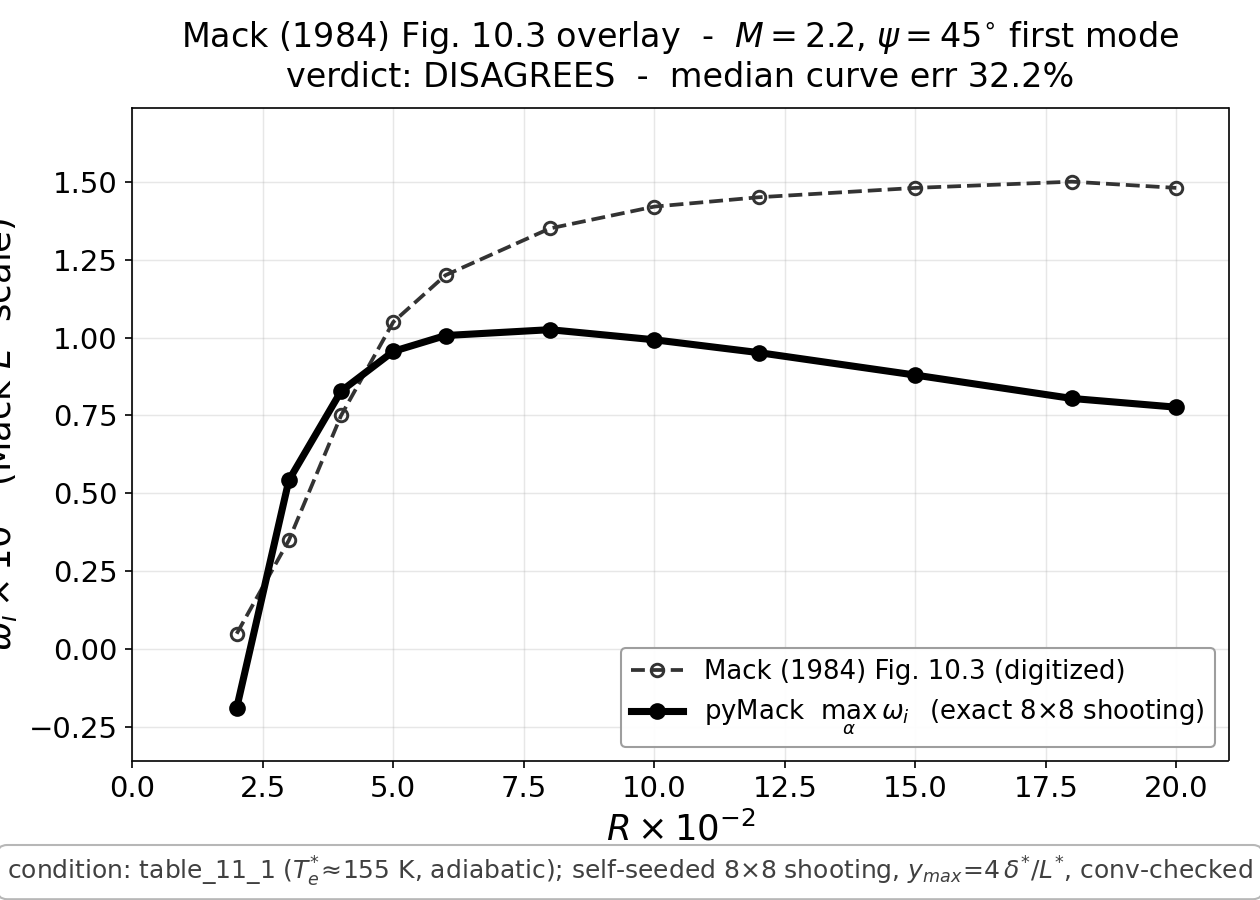
\includegraphics[width=0.72\linewidth]{../verification/first_mode/mack_fig10_3_m2p2/overlay.png}
\caption{Mack (1984) Fig.~10.3, $M=2.2$, $\psi=45^\circ$ (\emph{disagrees}):
correct topology but curve median $32.2\,\%$ --- the first-mode
under-amplification, confirmed convergence-stable.}
\label{fig:mack103_m22}
\end{figure}

\subsection{Mack (1984) Fig.~10.1 --- $M=2.2$ first-mode neutral loop}
\label{sec:mack101_m22}

\textbf{Reference source.} Mack (1984) AGARD-R-709, Fig.~10.1, the innermost
(Complete-Equations) neutral loop, $M=2.2$ (adiabatic, 2-D).

\textbf{Quantity compared.} The first-mode neutral loop (lower onset $+$ upper
cutoff branches) and the critical Reynolds number.

\textbf{Result --- \emph{disagrees}.} Loop-average median $|\Delta F|/F=54.5\,\%$,
critical $R$ pyMack $\sim\!400$ vs.\ Mack $\sim\!300$; the branch frequencies run
high and pyMack's loop is wider/higher than Mack's Complete loop --- its upper
branch overlies the Dunn--Lin numerical/asymptotic loops rather than the Complete
one. Even at the generous end of the $\sim\!5$--$12\,\%$ digitisation uncertainty
the gap is robust (the corrected reference already removed a prior reference-curve
error). The companion $M=1.6$ loop is \emph{acceptable} and is shown in the
validation note.

\remark{Confidence note.}{The Mack Fig.~10.1/10.3/10.4 first-mode cases are
computed through a reduced dense-EVP path
(\texttt{solve\_temporal\_compressible\_3d}) that has not yet had the discrete-mode
(eigenfunction-decay $+$ $y_{\max}$-stationarity) scrutiny already applied to the
\"Ozgen first-mode cases. The $M\approx2.2$ disagreement should be re-examined
under that path before it is treated as final; it is filed here as open.}

\FloatBarrier
\section{Incomplete engineering \& pipeline cases}
\label{sec:incomplete}

\bridge{These flight-relevant cases inherit the validated second mode, but each
carries an unfinished element: a bounded magnitude deficit (the cone $N$-factor),
a benchmark against an unpublished collaborator code, or a pure pyMack
self-consistency demonstration with no external reference.}

\subsection{Sharp cone --- Sivasubramanian (2012), Mach 6 second-mode $N$-factor}
\label{sec:cone}

\textbf{Reference source.} P.~Sivasubramanian (2012) PhD thesis, Univ.\ of
Arizona (hdl:10150/228514), Fig.~5.1 --- $N$-factor curves for axisymmetric
waves from a low-amplitude DNS wave-packet simulation on a sharp $7^\circ$ cone
at Mach 6 (BAM6QT); the linear parent of Sivasubramanian \& Fasel (2015)
\emph{J.\ Fluid Mech.} \textbf{768}:175--218. The thesis states verbatim that the
most-amplified axisymmetric wave reaches $N\approx9.5$ at $F=1.071\times10^{-5}$
($f^\ast\approx210$~kHz).

\textbf{Flow conditions.} Sharp $7^\circ$ half-angle cone, $M_\infty=6$,
isothermal $T_w=300$~K ($T_w/T_e=4.70$), axisymmetric ($\psi=0^\circ$).
Taylor--Maccoll edge state $M_e=5.356$, $T_e=63.78$~K, $U_e=857.5$~m/s;
Mangler path (transverse curvature omitted). $N$ integrated over the same
physical extent as thesis Fig.~5.1 (axial $x^\ast=0.30\to0.59$~m, from the lower
neutral point).

\textbf{Quantity compared.} The second-mode peak-$N$ frequency and the peak
linear $N$-factor.

\textbf{Result --- \emph{acceptable}, magnitude incomplete.} \textbf{Frequency:
exact.} pyMack's peak-$N$ frequency is $205$~kHz ($N=8.11$), i.e.\ $2.4\,\%$ from
the thesis $210$~kHz; evaluated \emph{at} $210$~kHz pyMack gives $N=8.05$ ---
pyMack independently reproduces $F=1.071\times10^{-5}$ as the most-amplified
frequency. \textbf{$N$-factor: $\sim\!15\,\%$ short.} pyMack $8.0$--$8.1$ vs.\
thesis $9.5$. The shape tracks the thesis well through $x^\ast\approx0.50$~m
(pyMack $6.5$ vs.\ $\sim\!6.6$), but the self-similar Blasius/Mangler local growth
rate decays faster than the cone DNS in the back half, so the last $\sim\!1.4$ of
$N$ is not accumulated --- the expected signature of omitting transverse curvature
and the real non-similar cone mean flow. The domain-matched $N=8.05$ is bracketed
by the BAM6QT design review (arXiv:2509.10411: $N\!\sim\!8$ at end of cone,
$\sim\!9$ at end of flare, $>\!10$ low-noise). \textbf{Open item:} closing the
$\sim\!1.4$-$N$ deficit needs a non-similar cone mean flow with transverse
curvature; until then the magnitude is bounded but not converged
(Figure~\ref{fig:cone}).

\begin{figure}[H]
\centering
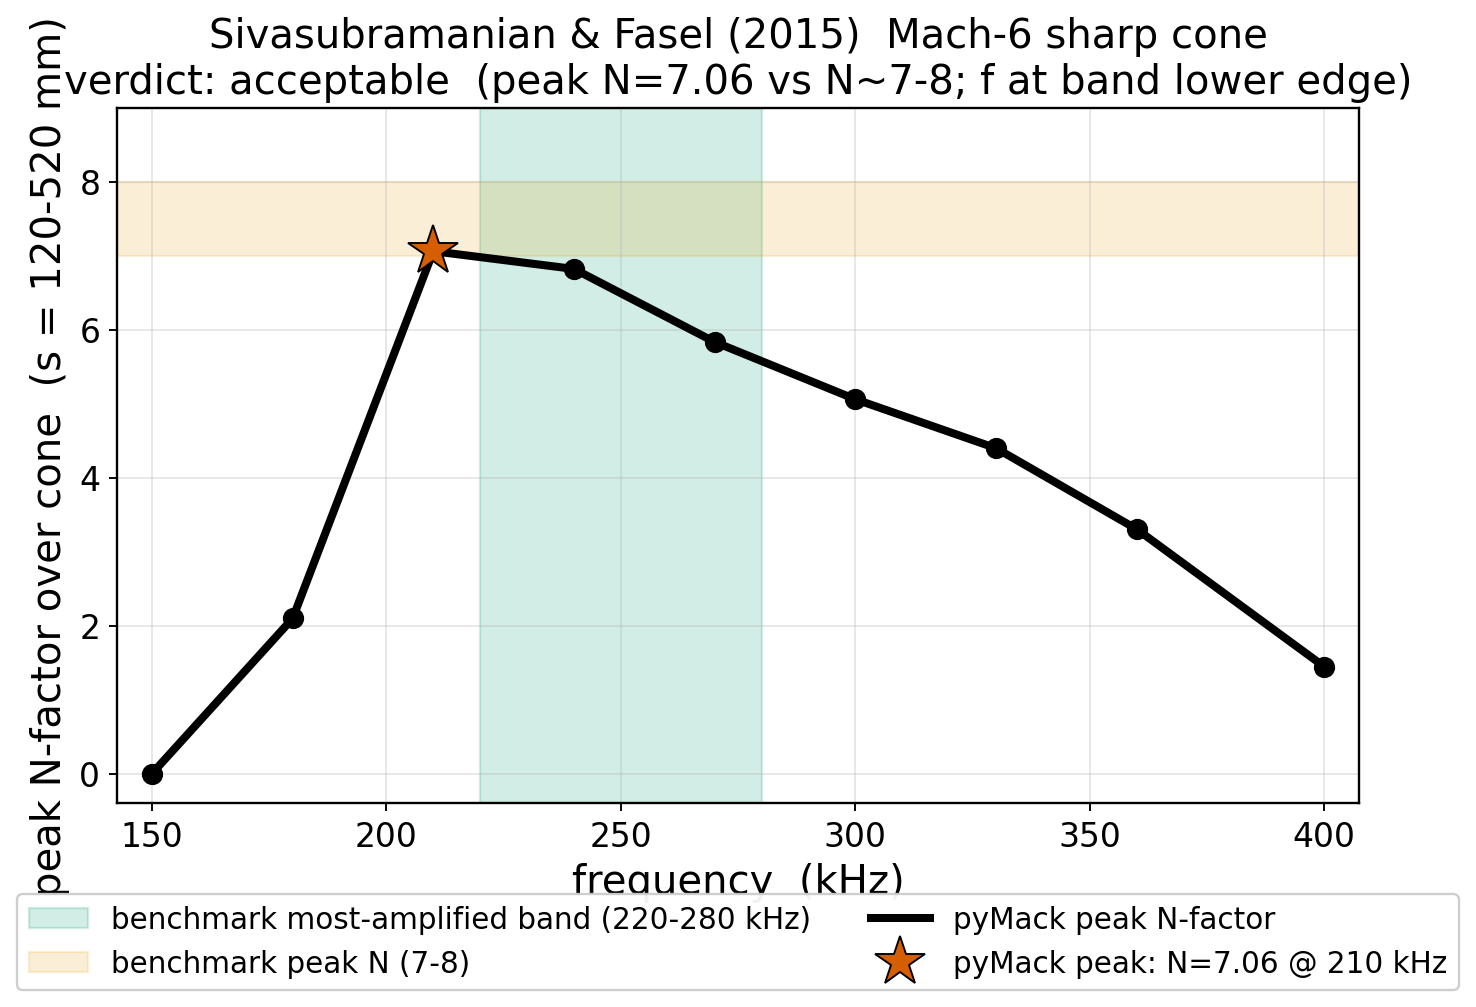
\includegraphics[width=0.72\linewidth]{../verification/second_mode/cone_sivasubramanian_fasel_2015/overlay.png}
\caption{Sharp $7^\circ$ Mach-6 cone, Sivasubramanian (2012) Fig.~5.1
(\emph{acceptable}, magnitude incomplete): pyMack second-mode $N$-factor vs.\ the
thesis. Frequency $210$~kHz matches exactly; peak $N\approx8.05$ vs.\ thesis $9.5$
($\sim\!15\,\%$ short) from the omitted transverse curvature / non-similar mean
flow.}
\label{fig:cone}
\end{figure}

\subsection{Collaborator Mach 5.35 nitrogen benchmark}
\label{sec:sean}

\textbf{Reference source.} An independent collaborator (``Sean'') LST code,
Mach 5.35 nitrogen neutral curve (unpublished; a code-to-code cross-check rather
than a literature anchor).

\textbf{Flow conditions.} $M=5.35$, $\psi=0^\circ$, nitrogen, adiabatic
($\sim\!370$~K wall); unit Reynolds number $1.176\times10^{7}$/m, edge velocity
$857$~m/s.

\textbf{Quantity compared.} The dimensional neutral-branch locations vs.\
frequency in mm (lower $=x_{\rm left}$, upper $=x_{\rm right}$). Dimensional
curves use MAE as a fraction of the curve span.

\textbf{Result --- \emph{acceptable}.} Upper branch MAE $3.21$~mm over
$200$--$600$~kHz (reference span $220.3$~mm $\Rightarrow$ \emph{agrees}); lower
branch MAE $1.29$~mm over $330$--$600$~kHz (span $19.8$~mm $\Rightarrow$
\emph{acceptable}); full $200^+$~kHz lower-branch MAE $6.68$~mm
(\emph{acceptable}). The two independent codes agree on the second-mode neutral
band to a few millimetres (Figure~\ref{fig:sean}). \textbf{Open items:} (i) this
is a private code-to-code comparison, kept out of the main note until it can be
tied to a published reference; (ii) the larger low-frequency lower-branch
residual (full $200^+$~kHz MAE $6.68$~mm) is a candidate
disturbance-temperature wall-BC mismatch --- pyMack uses the isothermal
$\hat{T}|_{w}=0$ condition, but the collaborator's disturbance-$T$ BC is
undocumented. This is exactly the adiabatic-vs-isothermal disturbance-BC
distinction that, when corrected, tightened the Ma \& Zhong and Malik case-3/5
comparisons; it cannot be resolved for this case without confirming which BC
Sean's code used. Pending that, the residual may be a convention difference
rather than a solver disagreement.

\begin{figure}[H]
\centering
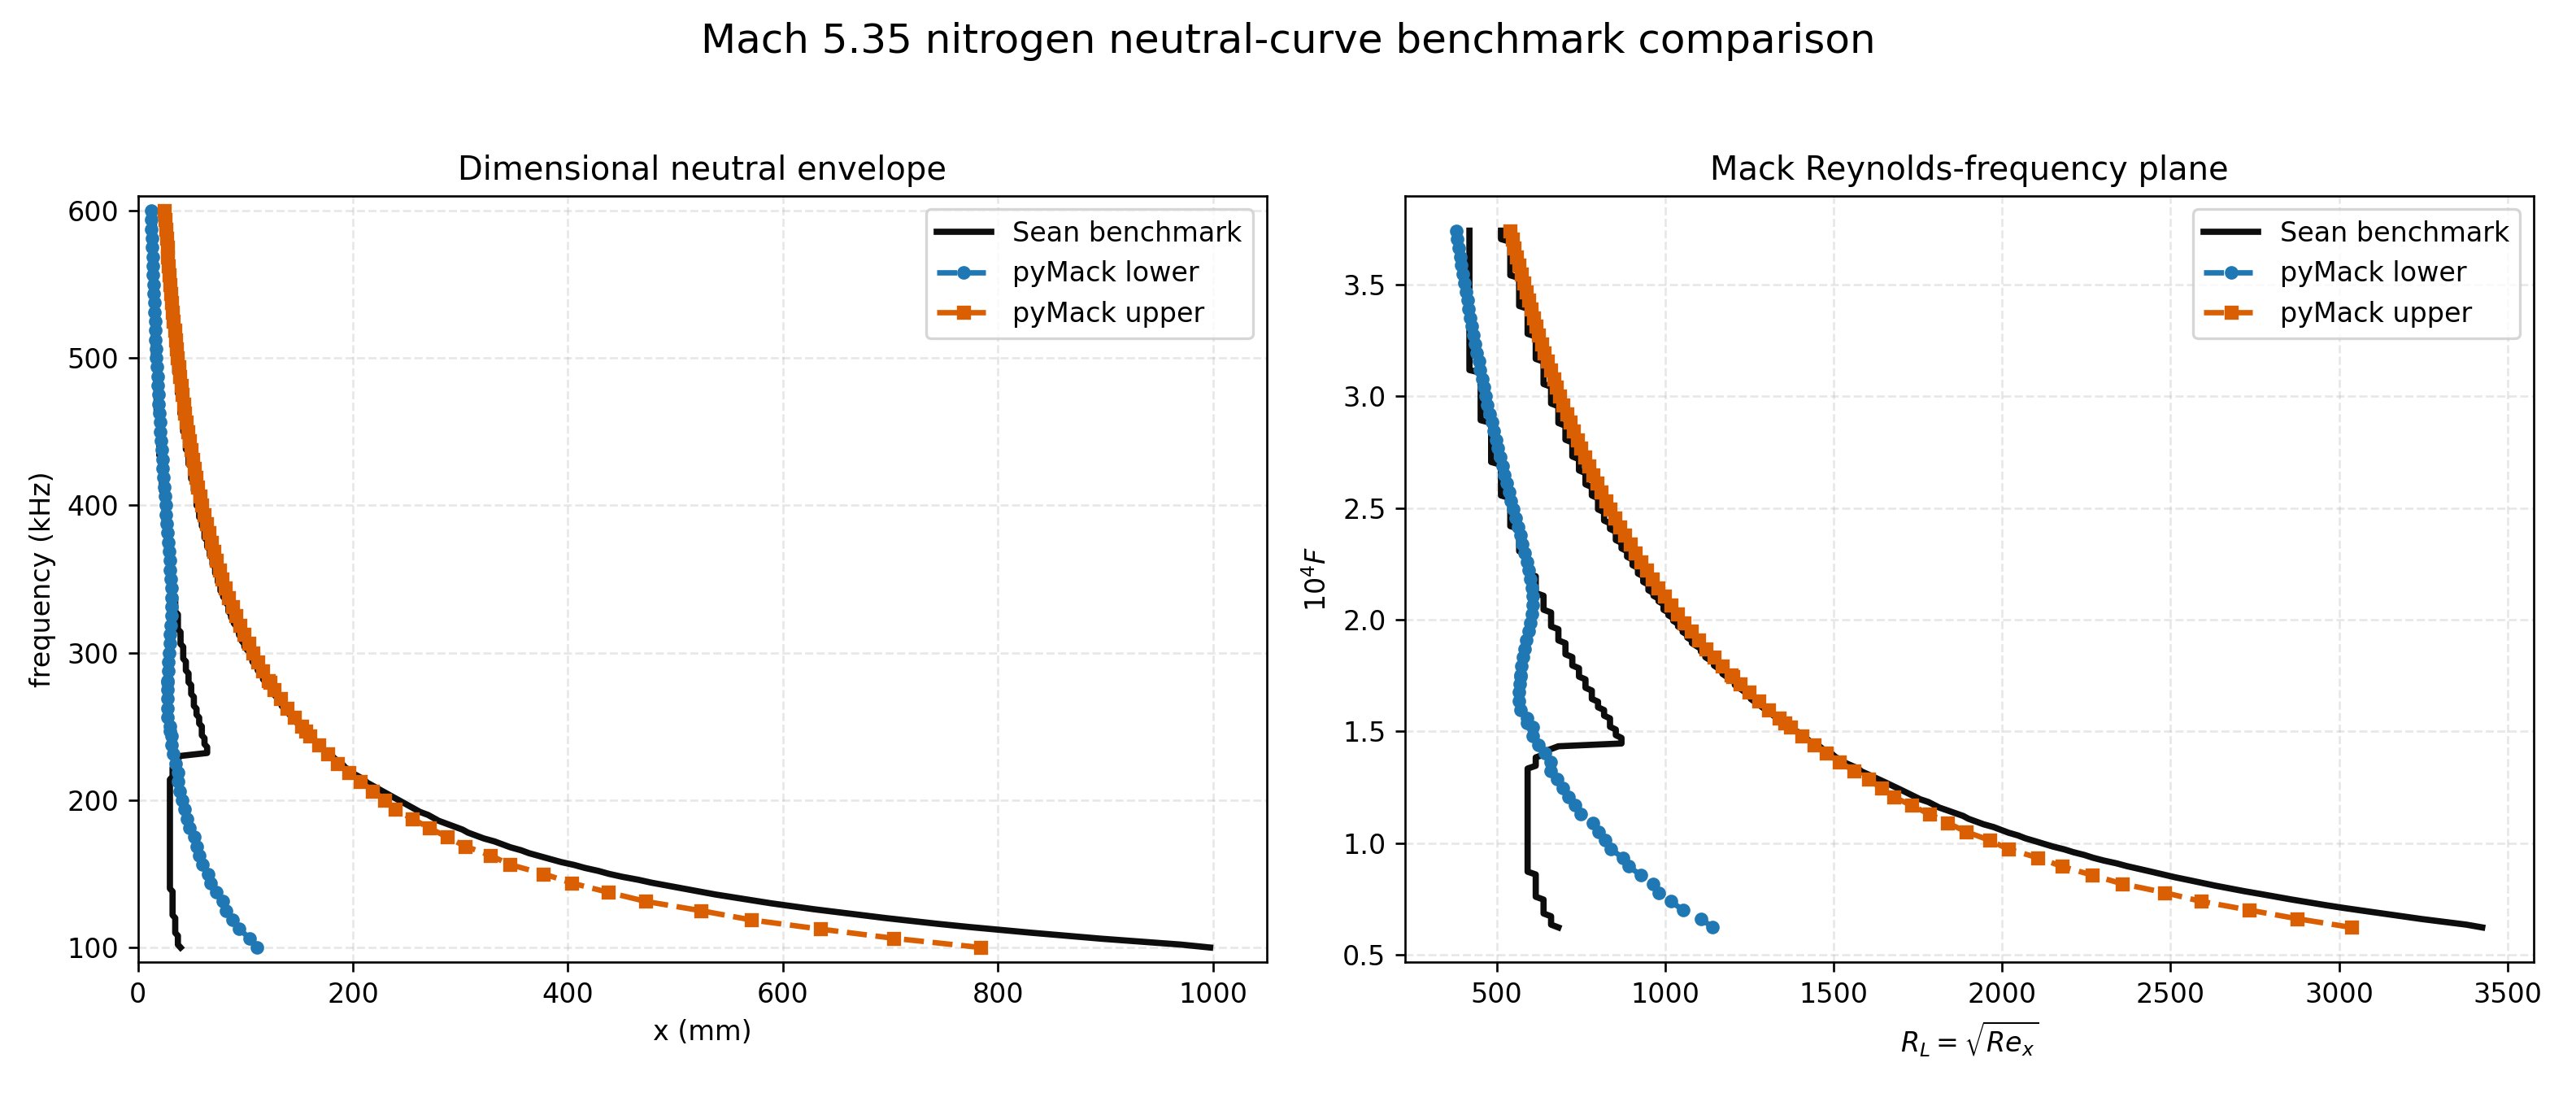
\includegraphics[width=0.72\linewidth]{mach5p35_collaborator_benchmark.png}
\caption{Mach 5.35 nitrogen: pyMack's neutral branches over the collaborator's
independent LST code. Upper-branch MAE $3.21$~mm, lower-branch MAE $1.29$~mm
(gated bands).}
\label{fig:sean}
\end{figure}

\subsection{Mach 6 spatial neutral curve and $N$-factor (pipeline demonstration)}
\label{sec:mach6pipeline}

\textbf{Purpose.} These two committed pyMack figures
(Figures~\ref{fig:mach6neutral} and \ref{fig:mach6nfactor}) demonstrate the full
spatial pipeline --- neutral-curve tracing and $N$-factor integration --- at a
representative Mach 6 flat-plate condition. They are pyMack self-consistency /
capability plots (no external reference overlay), included to show the
engineering deliverables the validated second mode feeds into. They are here
rather than in the validation note precisely because they are demonstrations, not
comparisons against a reference.

\begin{figure}[H]
\centering
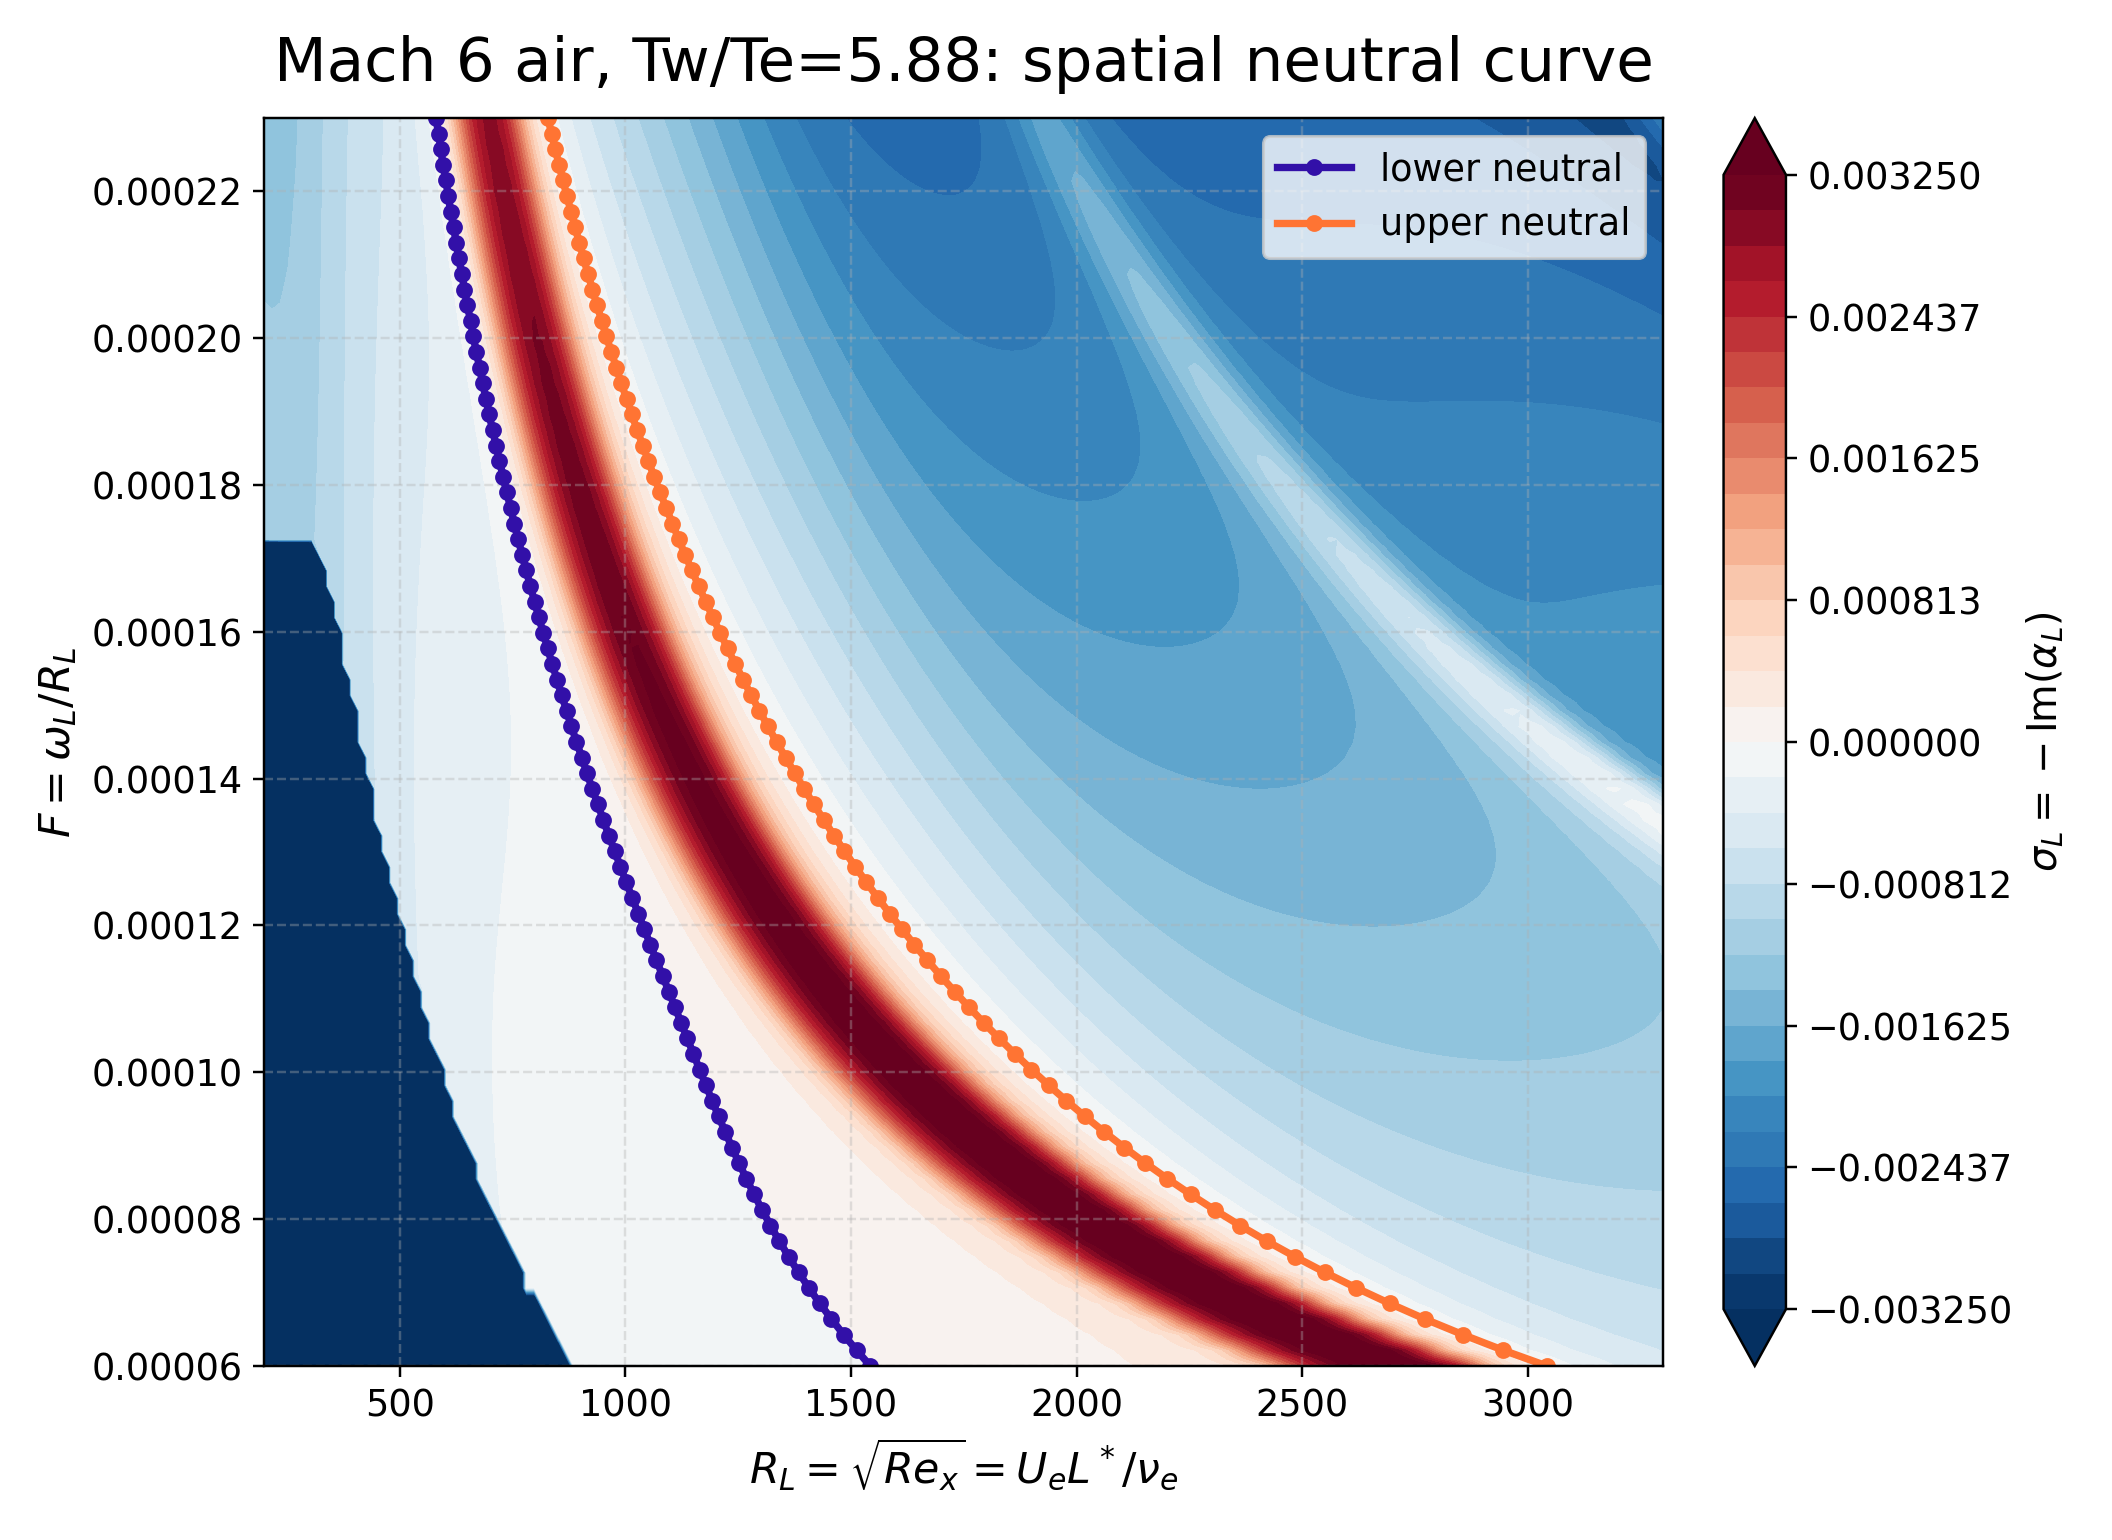
\includegraphics[width=0.72\linewidth]{mach6_spatial_neutral_curve.png}
\caption{Mach 6 spatial neutral curve produced by pyMack --- the second-mode
instability boundary in the frequency/streamwise plane, at a representative
Mach 6 flat-plate condition ($T_w/T_e=5.88$).}
\label{fig:mach6neutral}
\end{figure}

\begin{figure}[H]
\centering
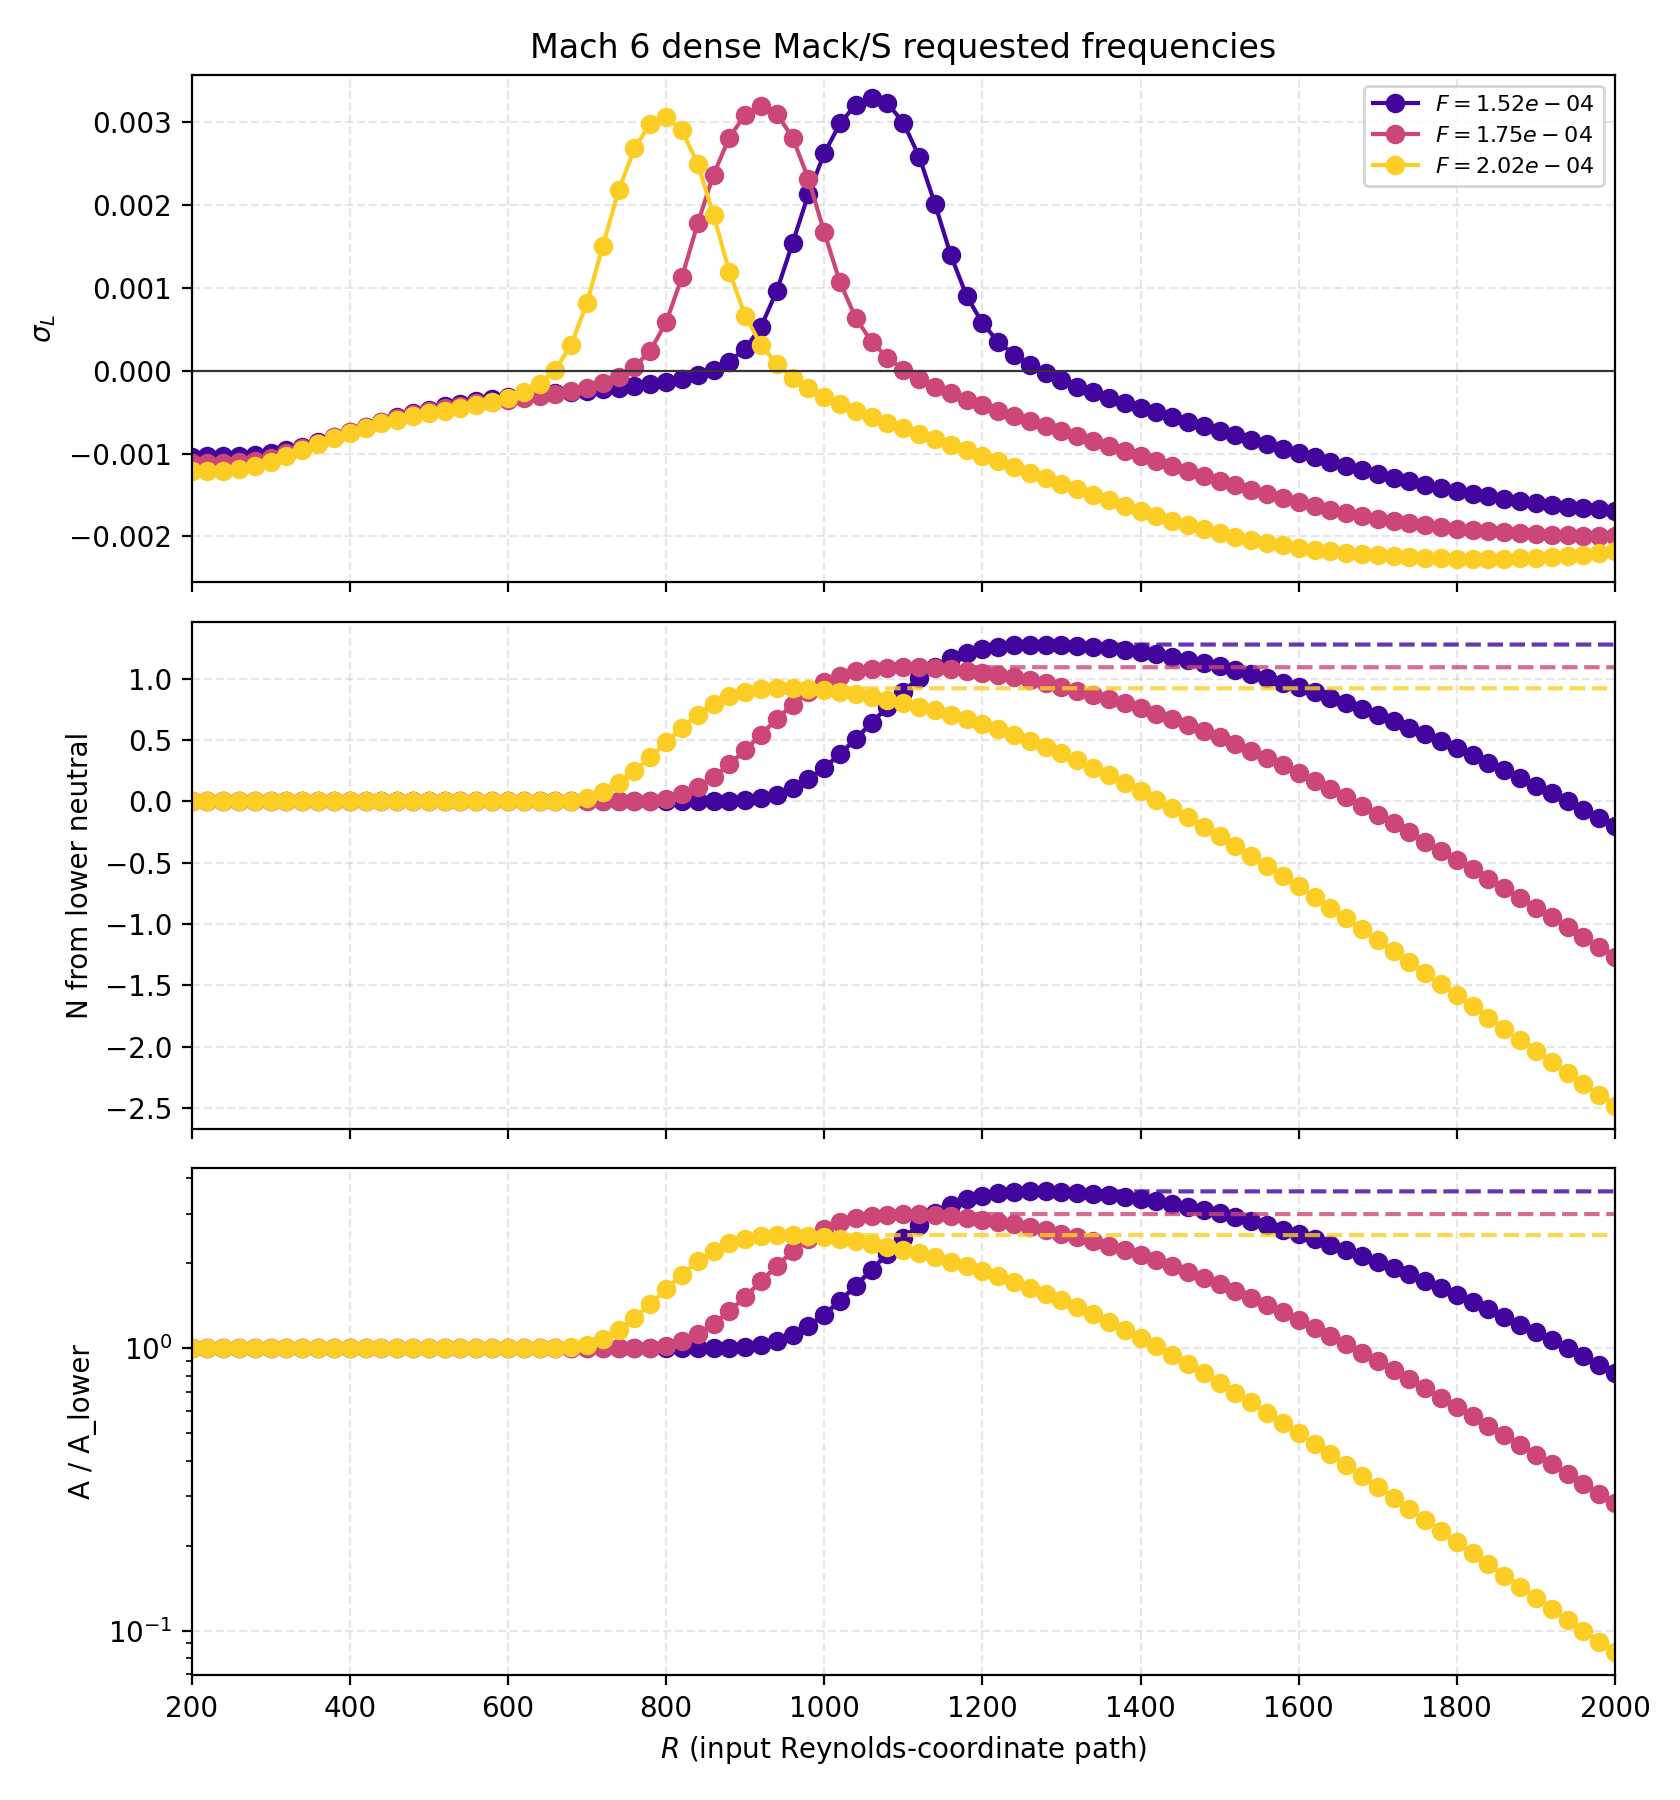
\includegraphics[width=0.72\linewidth]{mach6_growth_nfactor.png}
\caption{Mach 6 spatial growth rate and integrated $N$-factor from pyMack ---
the envelope quantity used for transition estimation.}
\label{fig:mach6nfactor}
\end{figure}

\FloatBarrier
\section{Method limitation: first-mode onset near the continuous spectrum}
\label{sec:cs-onset}

\bridge{This is a numerical-method boundary rather than a physics disagreement:
one \emph{part} of one validation curve --- the Ma \& Zhong $M=4.5$ first-mode
\emph{onset} branch --- lies where \texttt{pyMack}'s available solvers cannot
isolate a clean discrete mode. The second mode (the case's verdict) and the
first-mode cutoff branch are settled in the main note; only the onset branch is
open, and the cause is now understood.}

\subsection{Ma \& Zhong (2003) Fig.~15 --- $M=4.5$ first-mode onset branch}
\label{sec:mazhong-onset}

\textbf{What is settled (main note).} The $M=4.5$ second-mode neutral loop agrees
(branch points $2.4\,\%$/$1.0\,\%$), and the first-mode \emph{cutoff} (upper)
branch, re-extracted with the discrete-mode selector (freestream decay $+$
$y_{\max}$-stationarity), tracks Fig.~15 to $\sim\!3.5\,\%$.

\textbf{What is open.} The first-mode \emph{onset} (lower) branch --- Ma \&
Zhong's low-$\omega$ boundary, $\omega\approx0.006$--$0.043$ --- is not recovered.
Below $\omega\approx0.03$ the 2-D first mode's phase speed drops to
$c_r\!\lesssim\!0.45$, deep inside the slow-acoustic continuous spectrum
($c_r\le1-1/M=0.778$); there the discrete eigenmode delocalises (its eigenfunction
stops decaying at the freestream and becomes $y_{\max}$-sensitive), so no clean
discrete mode exists to trace.

\textbf{Robustness of the diagnosis.} The truncation is method-independent within
\texttt{pyMack}: the spatial collocation solver, the temporal collocation solver,
and a QR-orthonormalised shooting variant all recover the cutoff branch and all
lose the onset branch. The shooting variant, which imposes exact freestream decay,
finds the second mode cleanly (wall singular value $\sigma\!\to\!10^{-13}$) but has
\emph{no} zero at the first mode ($\sigma\approx0.18$, flat and
$y_{\max}$-independent) --- the parasitic-growth collapse of Gram--Schmidt shooting
when the freestream decay rates are poorly separated near the continuous spectrum.
A wave-angle sweep rules out the obvious alternative: the 2-D ($\psi=0$) mode is
the \emph{most} unstable at $M=4.5$ (peak temporal $c_i$ falls monotonically from
$1.2\times10^{-2}$ at $\psi=0$ to negative by $\psi\gtrsim60^\circ$), so Fig.~15's
first mode is 2-D, not oblique.

\remark{Path forward.}{Recovering the onset branch needs a \emph{compound-matrix}
(Plücker-coordinate) or Riccati shooting solver: by integrating the exterior
algebra of the bounded solution subspace it is immune to the parasitic-growth
collapse that defeats the QR shooting near the continuous spectrum. That is a
solver to build and validate (a few hundred lines), scoped here as a future item;
it is not required for any second-mode result.}

\end{document}
